% Created 2018-12-21 Fri 23:07
% Intended LaTeX compiler: pdflatex
\documentclass[letterpaper]{article}
\usepackage[utf8]{inputenc}
\usepackage[T1]{fontenc}
\usepackage{graphicx}
\usepackage{grffile}
\usepackage{longtable}
\usepackage{wrapfig}
\usepackage{rotating}
\usepackage[normalem]{ulem}
\usepackage{amsmath}
\usepackage{textcomp}
\usepackage{amssymb}
\usepackage{capt-of}
\usepackage{hyperref}
\usepackage{../src/mycv}
\usepackage{../src/config}
\author{Jaxson Van Doorn}
\date{\today}
\title{Resume Projects}
\hypersetup{
 pdfauthor={Jaxson Van Doorn},
 pdftitle={Resume Projects},
 pdfkeywords={},
 pdfsubject={},
 pdfcreator={Emacs 26.1 (Org mode 9.1.14)},
 pdflang={English}}
\begin{document}

\photo{images/profile.jpg} \resheader{ Jaxson Van Doorn }{jaxson.vandoorn.ca}{ jaxson.vandoorn@gmail.com }{ 250-508-2275 }{ 8636 Sentinel Place }{ North Saanich, BC }{ V8L 4Z8 }
\section{Projects}
\label{sec:orgd634bc6}
\subsection{\href{https://github.com/woofers/woofers3d}{Woofers 3D}}
\label{sec:orga5ac82a}
\subsubsection{Java}
\label{sec:org95c37a7}
\emph{Woofers 3D} is a Java API that attempts to unify the features of Box2D and Bullet Physics into a simple yet capable package that can be run on nearly any device via LibGDX. Supports modern features such as ray tracing, chasing camera, game states and 3D model importing.
\iffalse
\url{./images/woofers3d/1c.gif}
\fi
\subsection{\href{https://github.com/woofers/whale}{Whale}}
\label{sec:org20eadf2}
\subsubsection{Haxe}
\label{sec:org3435744}
\emph{Whale} is a 2D arcade style game built using HaxeFlixel. It features score tracking, level generation and responsive accelerometer controls. Game is fully completed and can be downloaded from the Google Play Store.
\iffalse
\begin{center}
\begin{tabular}{ll}
\begin{center}
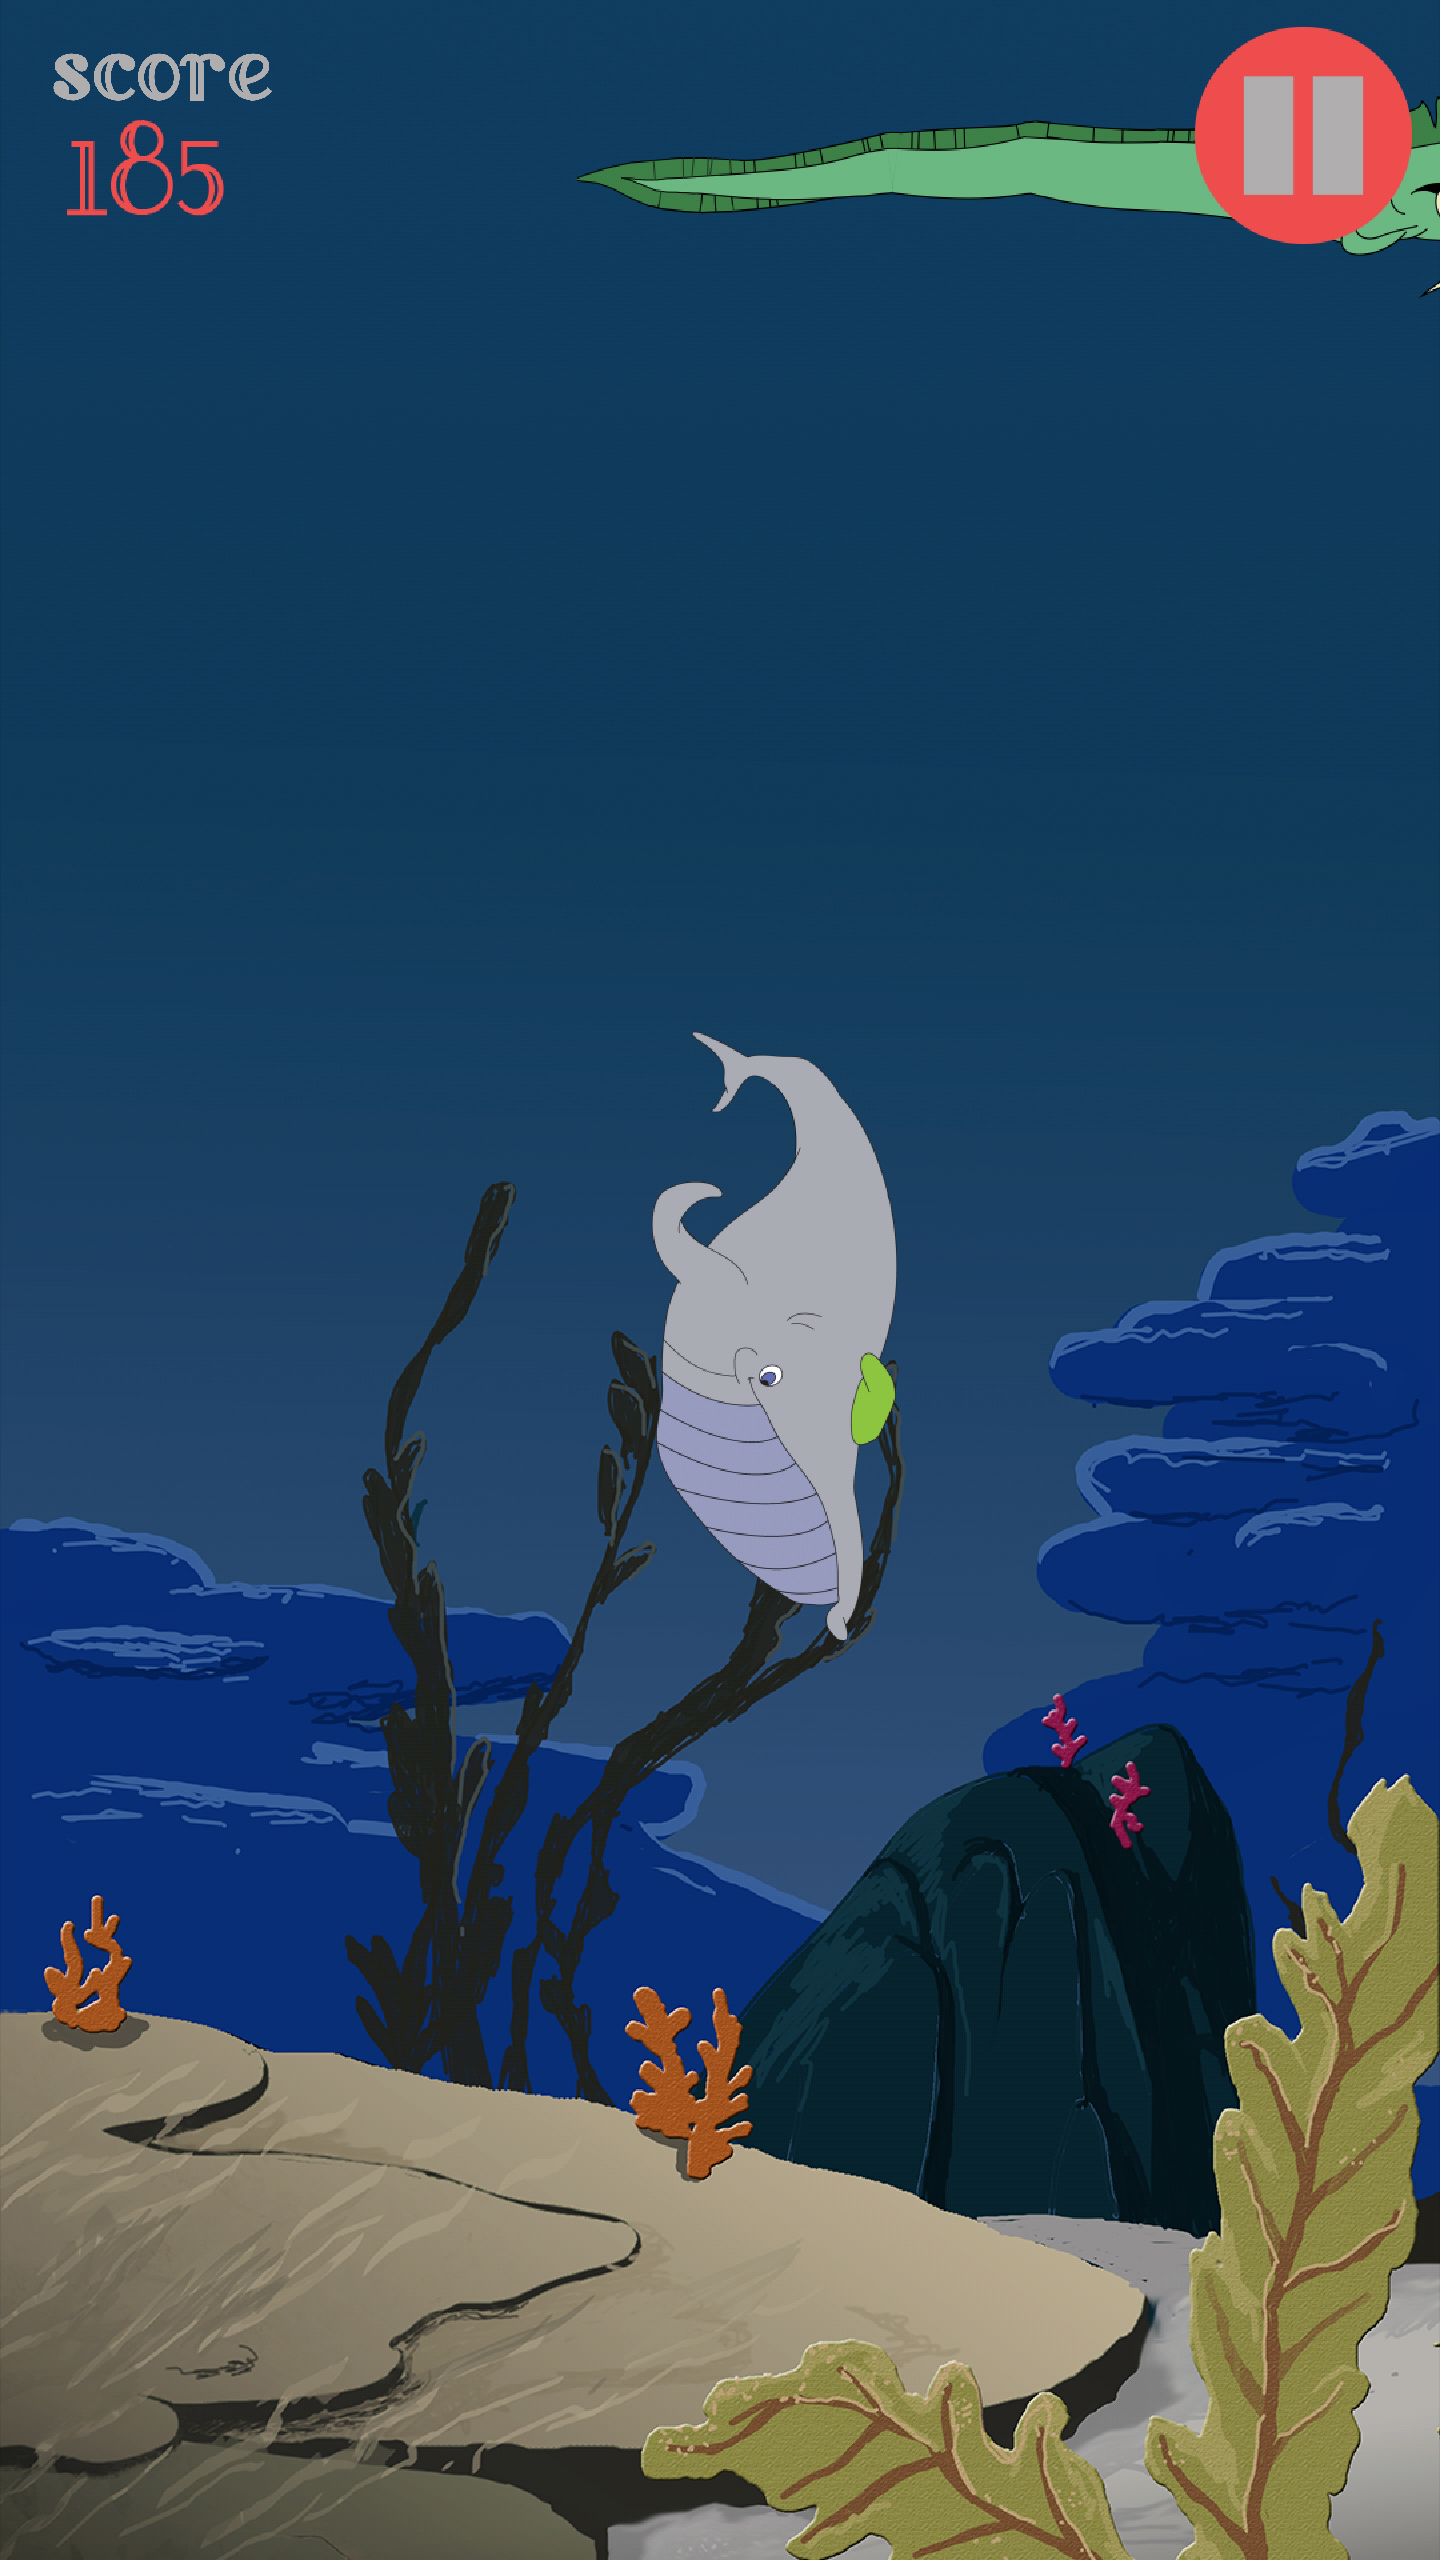
\includegraphics[width=.9\linewidth]{./images/whale/4.png}
\end{center} & \begin{center}
\includegraphics[width=.9\linewidth]{./images/whale/2.png}
\end{center}\\
\end{tabular}
\end{center}
\fi
\subsection{\href{https://github.com/woofers/kangaroo-country}{Kangaroo Country}}
\label{sec:org6012b1b}
\subsubsection{Actionscript 3}
\label{sec:orgae93b6c}
\emph{Kangaroo Country} is a 2D side-scrolling game built in Actionscrpt 3. Game features two fully completed levels where you play as two distinct characters in-order to solve platforming puzzles. As levels are imported from JSON based Tile Editor files, more levels can be dynamically added and created by others.
\iffalse
\begin{center}
\includegraphics[width=.9\linewidth]{./images/kangaroo/2.png}
\end{center}
\fi
\subsection{\href{https://github.com/woofers/fox-hole}{Fox Hole}}
\label{sec:org9121c95}
\subsubsection{Javascript}
\label{sec:org83720a4}
\emph{Fox Hole} is a 2D proof of concept game built in Javascript with Phaser. You play as a fox sneaking past enemy crocodiles using underground tunnels in order to save your brother. It features checkpoints and enemies complete with very basic AI.
\iffalse
\begin{center}
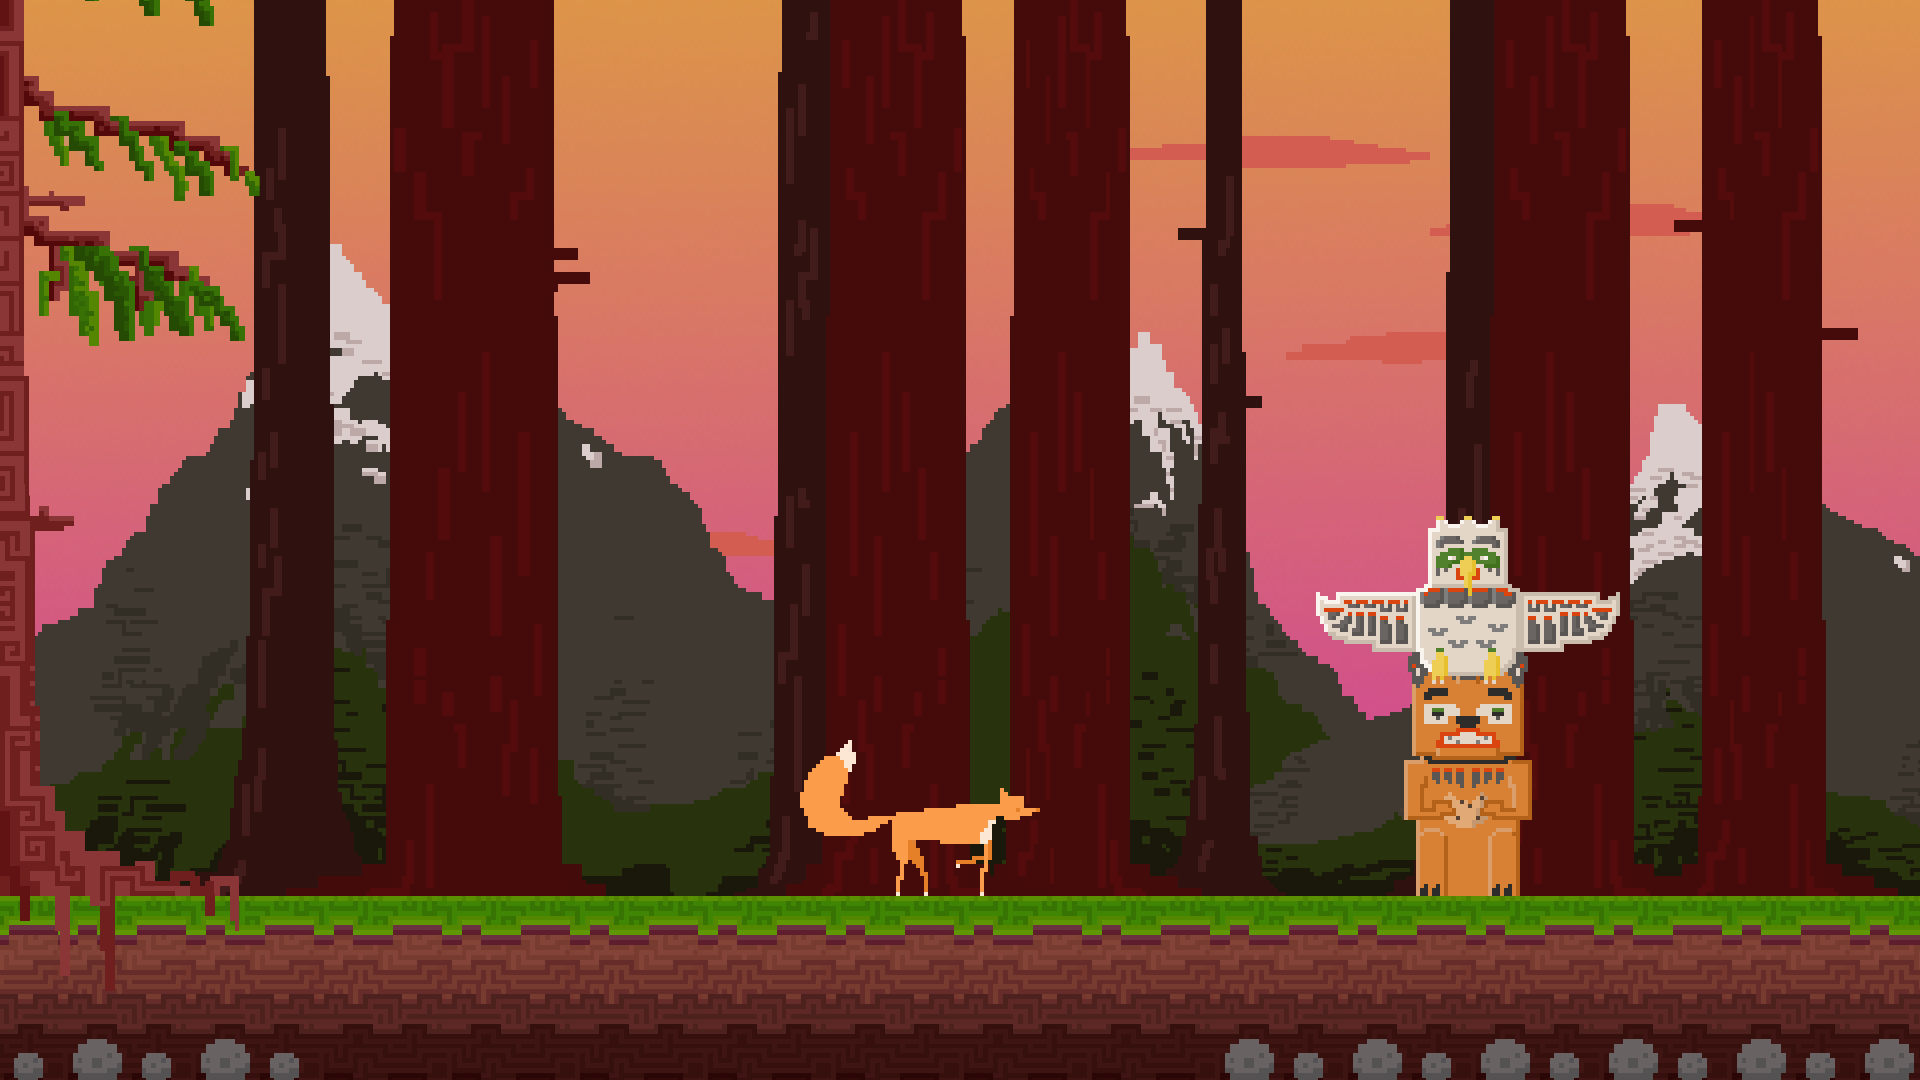
\includegraphics[width=.9\linewidth]{./images/fox/1.png}
\end{center}
\fi
\section{Skills}
\label{sec:org06c9ee3}
\begin{itemize}
\item Experience working with Java, Javascript, Actionscript 3, SQL, GraphQL and Git.
\item Ability to quickly adapt to new tools, work-flow and procedures.
\item Comfortable with both Windows, Linux and MacOS commandline tools and ecosystems.
\end{itemize}
\toggleurlstyle
\section{Experience}
\label{sec:org786fcd4}
\subsection{Software Developer Co-op at \href{https://ftsinc.com}{FTS Inc.}}
\label{sec:orga63c7a1}
\subsubsection{April 2018 - December 2018}
\label{sec:org1024c5a}
\textbf{Victoria, BC}
\begin{itemize}
\item Develop new features and services for web applications and APIs communicating with remote weather stations.
\item Configure, manage and version software projects using automated deployment tools.
\item Integrate Open Source tools used to configure IoT devices with existing software.
\end{itemize}
\section{Education}
\label{sec:org3c7813f}
\subsection{BSc, Computer Science at \href{https://uvic.ca}{University of Victoria}}
\label{sec:org7b99cb2}
\subsubsection{Sept 2017 - Present}
\label{sec:orge41b31d}
\textbf{Victoria, BC}
\begin{itemize}
\item Expecting Graduation in 2021
\end{itemize}
\end{document}
